\chapter{Nasadenie do vyučovania}
\label{chap:nasadenie_do_vyucovania}

Aby bola preverená celková kvalita virtuálneho laboratória, bol nástroj EVE-ng nasadený na vypracovávanie rôznych topológii z vybraných predmetov. 




\section{Používanie EVE-ng}
\label{chap:pouzivanie_eve_ng}

EVE-ng poskytuje na správu topológii a používateľov webové rozhranie. Webové rozhranie je dostupné v 2 módoch: natívnom a HTML5. HTML5 mód zabezpečuje integráciu pomocou reverzného proxy servera \emph{Apache Guacamole}, ktorý sa pripája na konzoly zariadení. HTML5 mód web rozhrania EVE-ng bol však menej stabilný a reagoval výrazne pomalšie pri práci s topológiou v provonaní s natívnym módom. Preto bolo webové rozhranie ďalej používané iba v natívnom móde.

V HTML5 móde sa na obrazovke s otvorenou topológiou po kliknutí na zariadenie otvorí jeho vzdialená konzola. V natívnom móde potrebujeme mať pre otvorenie konzoly na zariadení nainštalovaný tzv. integračný balíček. Predvolená vs KIS verzia integračného balíčka -> SSH tunely (pre vzdialený prístup k zariadeniam v topológii).


{\huge TODO - prekonzultovať, či stíham dopísať túto kapitolu}

-popisat
      -vytvorenie topologie
        -z GUI (pridavanie zariadenia)
        -editovaním UNL súboru s topológiou
            -popisat hlavne parametre, ktore sa lisia pri duplikovani textovej reprezentacie danej topologie
        -vyslovit odporucanie na vytvaranie topologii
            -> GUI -> Nodes (nazvy zariadeni) -> UNL (skraslenie topologie upravenim suradnic pre zariadenia) - VID A4 PAPIER "DUPLIKÁCIA TOPOÓGIE V EVE-NG -> ZÁVER"
      -pridelovanie portovych cisel zariadeniam
        -rozsah
        -pridelovanie portovych cisel je sekvencne
      -spustanie zariadeni
        -po jednom
        -vybrana skupina
          -Ctrl+klik -> pravy klik -> Start Selected
          -oznacenie mysou -> pravy klik -> Start selected
        -vsetky zariadenia v topologii
          -More actions -> Start all nodes
      -odhadnut systemove poziadavky pre topologie z vybranych predmetov a na zaklade toho odhadnut minimalne systemove poziadavky servera
      -> začať topológiami z predmetov, na ktorých bol nástroj nasadený.




\section{Počítačové siete 2}

V rámci predmetu Počítačové siete 2 bol nástroj EVE-ng nasadený do vyučovania na vypracovávanie topológii s \emph{point-to-point} technológiami. Topológie boli spustené na fyzickom EVE-ng serveri. V prípade zlyhania EVE-ng boli pripravené aj záložné topológie v overenom nástroji Dynamips/Dynagen.

Najprv bola vytvorená základná topológia, znázornená na obrázku \ref{obr:eve_ng_ppp_zakladna_topo_v2}. Tá pozostávala zo štyroch Cisco IOL smerovačov a dvoch koncových zariadení s operačným systémom Alpine Linux. Cisco IOL smerovač bol vybraný, pretože ako jediný podporoval sériové rozhrania a \emph{point-to-point} technológie. Koncové zariadenie Alpine Linux bolo vybrané pre svoju nenáročnosť na systémové zdroje.

\begin{figure}
    \centering
    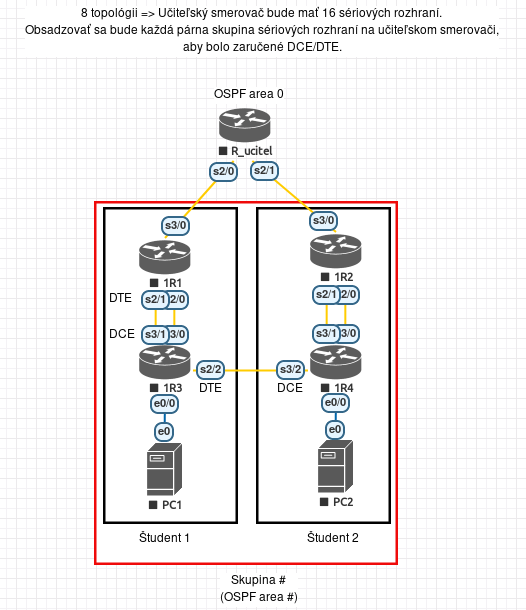
\includegraphics[width=0.75\textwidth]{eve_ng_ppp_zakladna_topo_v2}
    \caption{Základná PPP topológia}
    \label{obr:eve_ng_ppp_zakladna_topo_v2}
\end{figure}

Celkovo bolo vytvorených 8 zhodných topológii, ktoré medzi sebou zdieľali jeden učiteľský smerovač. V topológii sa celkovo nachádzalo 33 Cisco IOL smerovačov a 16 koncových staníc. Celková topológia sa nachádza na obrázku \ref{obr:eve_ng_ppp_celkova_topo_v2}.

\begin{figure}
    \centering
    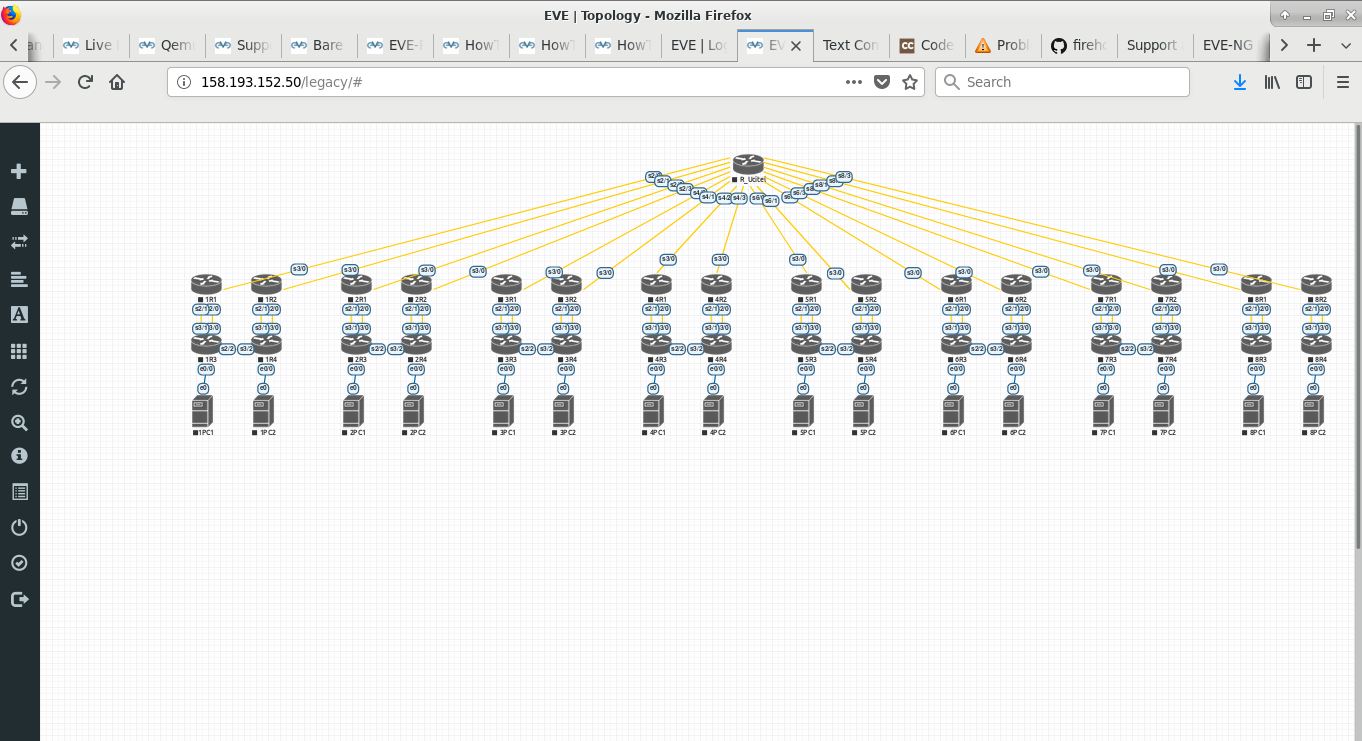
\includegraphics[width=0.75\textwidth]{eve_ng_ppp_celkova_topo_v2}
    \caption{Celková PPP topológia}
    \label{obr:eve_ng_ppp_celkova_topo_v2}
\end{figure}

IOL smerovače fungovali, až na príkaz \texttt{clock rate} na sériových rozhraniach, bez chyby. Ukázalo sa, že nastavenie DCE/DTE závisí od párnosti čísla skupiny. Párne číslo skupiny sériových rozhraní bude vždy DTE, nepárne vždy DCE, ako je zrejmé z obrázku \ref{obr:eve_ng_dce_dte_2E8S}. Rozdelenie sériových rozhraní na DCE/DTE nezávislé od počtu ethernetových alebo sériových skupín, čo potvrdzuje obrázok \ref{obr:eve_ng_dce_dte_1E8S}. Nanešťastie nastavenie DTE/DCE módu pre sériové rozhrania nie je v EVE-ng pri Cisco IOL smerovačoch automatické. {\huge TODO - Je automatické v Dynamips/Dynagene?}

\begin{figure}
    \centering
    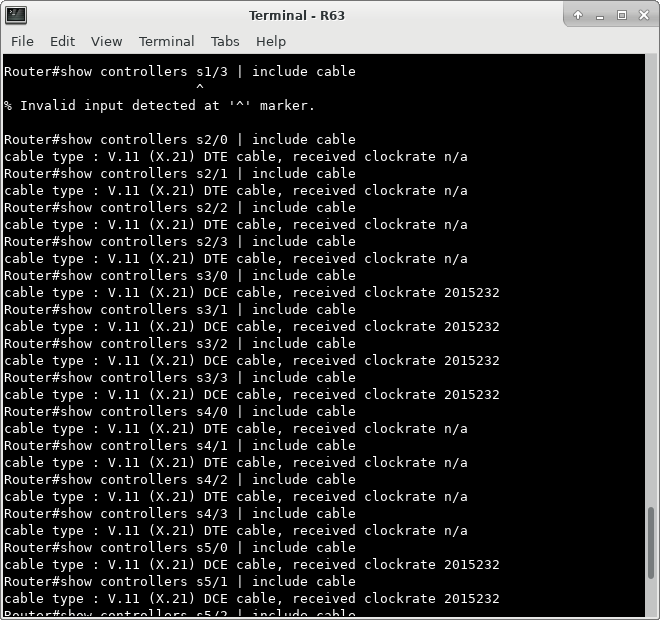
\includegraphics[width=0.75\textwidth]{eve_ng_dce_dte_2E8S}
    \caption{Typy sériových rozhraní na IOL smerovači - 2 ethernetové + 8 sériových skupín}
    \label{obr:eve_ng_dce_dte_2E8S}
\end{figure}

\begin{figure}
    \centering
    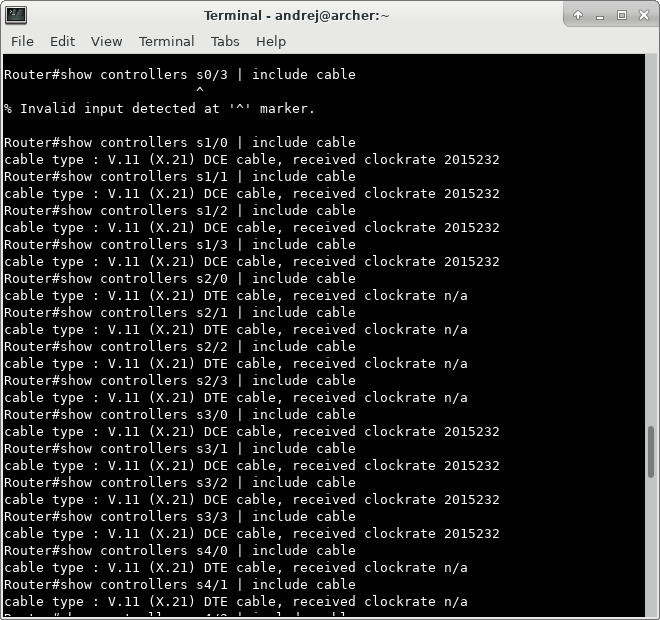
\includegraphics[width=0.75\textwidth]{eve_ng_dce_dte_1E8S}
    \caption{Typy sériových rozhraní na IOL smerovači - 1 ethernetová + 8 sériových skupín}
    \label{obr:eve_ng_dce_dte_1E8S}
\end{figure}

V jednej skupine sa vyskytol problém s jednosmernou PAP autentifikáciou študentského smerovača voči učiteľskému (R\_Ucitel(s4/1)-5R2(s2/1)). Príkaz \texttt{debug ppp authentication} hlásil chybu pri autentifikácii. Riešenie spočívalo v odstránení používateľa, vypnutí \emph{ppp} konfigurácie a vypnutí rozhraní. Tieto kroky boli vykonané aj na učiteľskom, aj na študentskom smerovači. Následne sa konektivita obnovila a spojenie pomocou PAP autentifikácie sa úspešne nadviazalo.

Je možné, že problémy vznikli aj kvôli tomu, že medzi študentským a učiteľským smerovačom boli na oboch stranách sériové rozhrania párnej skupiny t.j. obidva konce linky boli typu DTE. Niektoré skupiny študentov boli tiež pripojené k učiteľskému smerovaču sériovým rozhraním z párnej skupiny, ale takéto problémy nezaznamenali. Podobne tomu bolo aj pri prepojení Cisco IOL smerovačov rozhraniami DCE.

Z toho vyplýva, že Cisco IOL smerovače v EVE-ng majú pri prepojení dvoch smerovačov sériovou linkou s rovnakým módom nedefinované správanie. Tomu sa dá predísť vhodným návrhom topológie. Ten spočíva v tom, že sériové rozhrania medzi smerovačmi kombinujeme tak, aby bolo prepojené vždy sériové rozhranie párnej skupiny na jednom smerovači so sériovým rozhraním nepárnej skupiny na inom smerovači t.j. \emph{Serial2/x} (DCE) na prvom smerovači sa musí pripojiť napr. k \emph{Serial3/x} na druhom. V takom prípade DCE koniec po nastavení \texttt{clock rate} v príkaze \texttt{show controllers} zobrazí nastavený atribút \emph{received clockrate}, DTE koniec naproti tomu zobrazí hodnotu \emph{n/a}. Napriek tomu konektivita po správnom nastavení IP adries a zapnutí rozhranií bola aktívna.

Komplikácie s DCE/DTE a PPP autentifikáciou boli prítomné v prvom návrhu topológie, ktorý je znázornený na obrázku \ref{obr:eve_ng_ppp_zakladna_topo_v1}.

\begin{figure}
    \centering
    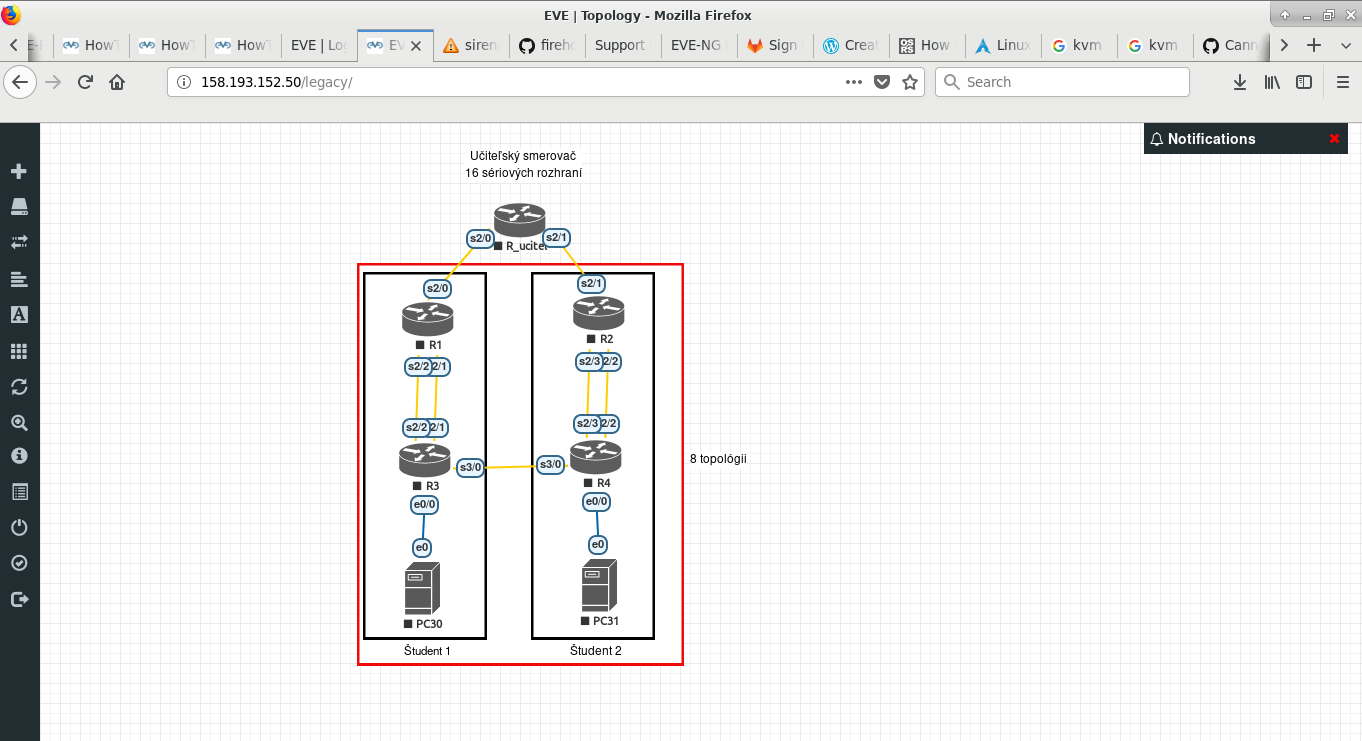
\includegraphics[width=0.75\textwidth]{eve_ng_ppp_zakladna_topo_v1}
    \caption{Základná PPP topológia - prvotný návrh}
    \label{obr:eve_ng_ppp_zakladna_topo_v1}
\end{figure}

Pri testovaní DCE/DTE rozhraní sme narazili na obmedzenie nástroja EVE-ng. Community verzia je totiž dovoľuje v jednej topológii mať spustených najviac 63 zariadení. Po spustení 64. sa na niekoľko sekúnd spustí, ale nakoniec sa automaticky vypne. Community verzia vie spustiť aj viac ako 64 zariadení v jednej topológii, ale vo výsledku sa spustia len niektoré, na prvý pohľad náhodne vybrané zariadenia. Avšak tie zariadenia, ktoré sa spustia, pracujú štandardným spôsobom. Uvedený problém sa nám nepodarilo vyriešiť ani rozšírením rozsahu portových čísel pre zariadenia v topológii.
  
Zmerané boli aj systémové požiadavky celkovej topológie na fyzickom EVE-ng serveri. Po vyhodnotení výsledkov merania sme zistili, že celá topológia, 33 Cisco IOL smerovačov a 16 koncových zariadení Alpine Linux, sa spúšťala približne 2 minúty, spotrebovala 13GB operačnej pamäte a procesor vyťažovala na 21\%. Celkovo by sme podľa celkového vyťaženia CPU mohli spustiť 4 takéto topológie, avšak množstvo operačnej pamäte dovoľovalo spustiť iba 3. Tabuľkový dokument s výsledkami merania je prítomný na CD v adresári \\ \emph{materialy\_na\_predmety/nasadenie\_do\_vyucovania/PS2/} v súbore \\ \emph{ps2\_7\_tyzden\_ppp\_topologia\_final\_8\_replik\_33\_IOL\_L3\_a\_16\_QEMU\_Alpine\_Linux.ods}.

Spomenutý súbor ukazuje veľké rozdiely v meraniach využitia operačnej pamäte medzi nástrojmi \emph{ps} a \emph{ps\_mem} v hárku \emph{VstupVystup}, hoci sa merala rovnaká množina procesov. Po manuálnom overení sa ukázalo, že prvý menovaný nástroj vykazoval presnejšie výsledky, preto boli pri odhadoch použité ním namerané hodnoty.





\section{Projektovanie sietí 2}

V rámci predmetu Počítačové siete 2 bol nástroj EVE-ng nasadený do vyučovania na vypracovávanie topológii s \emph{point-to-point} technológiami. Topológie boli spustené na virtuálnom VMware EVE-ng serveri.

V EVE-ng boli úspešne dokončené semestrálne práce s témou \emph{VPLS} a \emph{Seamless MPLS}. Téma \emph{EVPN} bola vypracovávaná v nástroji \emph{ViRo v2} 

Topológie semestrálnych prác sa skladali z týchto zariadení:

\begin{itemize}
    \item Cisco IOL smerovač - VPLS, Seamless MPLS
    \item Cisco CSR - VPLS
    \item Juniper Olive - Seamless MPLS
    \item Juniper vMX 15 - VPLS
    \item Nokia VSR - EVPN
\end{itemize}

{\huge TODO- replikovať jakubovu topológiu v EVE-ng - konfiguráky => FB, topológia => gmail konverzácia}


\section{Vyhodnotenie}

Z predmetov Počítačové siete 1, Pokročilé prepínanie v informačno-komunikačných sieťach a Pokročilé smerovanie v informačno-komunikačných sieťach neboli vypracované žiadne topológie.

Na predmetoch, kde nástroj EVE-ng nasadený bol, sa ukázalo, že ho je možné používať vo vyučovaní.

Študenti počas vypracovávaní topológie na predmete Počítačové siete 2 nezaznamenali žiadny rozdiel oproti nástroju Dynamips/Dynagen, keďže sa na zariadenia prihlasovali rovnako, pomocou nástroja \emph{PuTTY} IP adresou a portom, pričom zariadenia poskytovali rovnakú množinu funkcii, ako v nástroji Dynamips/Dynagen. Nástroj EVE-ng na fyzickom serveri bol počas celej doby vypracovávania stabilný.

Pri nasadení na predmet Projektovanie sietí 2, kde bola použitá virtuálna inštalácia EVE-ng, bol naopak nástroj nestabilný, zariadenia často zamŕzali a pri zadávaní príkazov do konzoly bola prítomná vyššia odozva z klávesnice. Mohlo to byť spôsobené mnohými faktormi, či už samotnou virtuálnou platformou VMware, alebo nesprávne nastavenými systémovými parametrami pre jednotlivé zariadenia v topológii.